\documentclass[11pt]{article}

\usepackage[margin=1in]{geometry}
\usepackage{amsmath}
\usepackage{amssymb}
\usepackage{graphicx}
\usepackage{xcolor}
\usepackage{titlesec}
\usepackage[hidelinks]{hyperref}
\usepackage{parskip}
\usepackage{enumitem}
\usepackage{booktabs}

\definecolor{linknavy}{RGB}{20,40,90}
\hypersetup{colorlinks=true, urlcolor=linknavy, linkcolor=linknavy}
\titleformat{\section}{\large\bfseries}{\thesection}{0.6em}{}
\titlespacing{\section}{0pt}{1.4em}{0.5em}
\titleformat{\subsection}{\normalsize\bfseries}{\thesubsection}{0.6em}{}
\newcommand{\code}[1]{\texttt{\small #1}}
\setlist{itemsep=1pt, topsep=3pt}
\sloppy
\emergencystretch=2.5em

\title{\vspace{-2.2em}\textbf{diffusion-tinker: technical walkthrough}}
\author{Srijit Iyer}
\date{Current as of the corrected reruns, July 2026}

\begin{document}
\maketitle
\vspace{-1.2em}

\noindent\textit{This is the standalone deep dive on diffusion-tinker, built from
first principles and kept current. It supersedes the diffusion-tinker section of
the resume walkthrough: the code is now fixed, the grid has been rerun, and one
result I published earlier (``DDRL collapses without an anchor'') turned out to be
my own bug, corrected here. Read Sec.~0 first, then whatever you want to go deep on.}

\section{How to use this document (read first)}

The honest framing, up front, because a senior researcher will find the soft spots
anyway and getting ahead of them reads as maturity.

\begin{itemize}
\item \textbf{It's co-authored.} \code{pyproject.toml} lists me plus \textbf{Haotian Ye}
and \textbf{Jiaqi Han} (Stefano Ermon's lab at Stanford). The SDE log-prob math in
\code{noise\_strategy.py} and the per-prompt stat tracker are adapted from FlowGRPO's
implementation, not derived from scratch. My contribution is the six trainers behind
one API, and finding and fixing the correctness bugs that made them actually train.
\item \textbf{The old ``0.950 vs 0.823'' number is dead.} That was measured before a
VAE decode-range bug, on images that were $\sim$55\% black. On fixed code the OCR
reward reaches 1.0, but eval is on training prompts (in-distribution), so it's a
``the-pipeline-works'' number, not a held-out benchmark. Don't claim I beat the paper.
\item \textbf{I corrected my own published result.} An earlier grid of mine showed
DDRL collapsing without a data anchor and concluded ``the KL anchor is more robust
than the data anchor.'' That was wrong. It was one flag set the wrong way
(\code{use\_monotonic\_transform=True}), which manufactured the collapse. With it off,
DDRL($\beta{=}0$) is the same update as FlowGRPO($\beta{=}0$) and nothing collapses.
Sec.~6 and Sec.~9 tell that story straight. Finding and reporting my own bug is the
part I'd lead with.
\item \textbf{No held-out eval, single runs, single GPU.} Every metric is on training
prompts; no error bars over seeds; not distributed. That's the honest ``what I'd fix
next.''
\end{itemize}

\section{The 30-second story}

diffusion-tinker is an open-source library for RL post-training of diffusion models
- think RLHF, but for image generators instead of LLMs (``post-training'' = extra
training applied after the base model is already trained). It gives a TRL-style API
(the same call shape as HuggingFace's TRL library) over HuggingFace Diffusers, and
implements six methods (FlowGRPO, DDPO/DPOK, DDRL, DiffusionDPO, DRaFT, SFT) behind
one \code{Trainer}/\code{Config} surface. Targets SD3.5 and FLUX.1.

The flagship is FlowGRPO on SD3.5, pushing the model to render legible text using OCR
as the reward: read the generated image, and if the text is spelled right the model
gets a high score. My biggest hands-on contribution was getting the training to
actually move a reward - which took finding several correctness bugs that only show
up when you check gradients and pixels on real GPUs, not in a smoke test.

\section{Foundations from scratch}

\subsection{What a diffusion model is, in one breath}

A diffusion model generates an image by \textbf{starting from pure noise and removing
a little noise at a time}, over many steps, until an image emerges. It's trained by
doing the opposite: take real images, add noise in steps, and teach a network to
predict and undo that noise. ``Noise'' here means random Gaussian pixel values, i.e.
random static.

\subsection{Forward process (fixed, no learning)}

Take a clean image \code{x\_0} and repeatedly add Gaussian noise until, after $T$
steps, it's indistinguishable from static \code{x\_T}:
\[
x_t = \sqrt{\bar\alpha_t}\, x_0 + \sqrt{1-\bar\alpha_t}\,\epsilon, \qquad \epsilon\sim\mathcal N(0,I)
\]
where $\bar\alpha_t$ (``a-bar sub t'') is the cumulative fraction of the clean image
that still survives at step $t$: near 1 early (little noise), near 0 late (all noise).

\subsection{Reverse process (the learned part)}

Start at noise \code{x\_T} and step back down to \code{x\_0}. A network predicts how
to denoise at each step. Classic DDPM (the original 2020 formulation) trains it as a
plain regression against the noise that was added:
\[
\mathcal L = \mathbb E \,\lVert \epsilon - \epsilon_\theta(x_t, t)\rVert^2
\]
$\epsilon_\theta$ is the network's predicted noise; $\theta$ its trainable weights.
Noise-prediction and the ``score'' (the gradient of the log data-density, the
direction in pixel space toward more image-like regions) are the same thing up to a
scale: $\text{score} = -\epsilon_\theta / \sqrt{1-\bar\alpha_t}$.

\subsection{The ODE $\leftrightarrow$ SDE duality (the single most important idea for FlowGRPO)}

The whole denoising process can be written as a continuous differential equation.
There are two forms that produce the \textbf{same distribution of images}:
\begin{itemize}
\item \textbf{ODE (deterministic):} same noise in $\to$ same image out, every time.
Fast, reproducible.
\item \textbf{SDE (stochastic):} injects fresh randomness at each step. Same final
distribution, but the path wanders.
\end{itemize}
Why you care: RL needs randomness to explore (try different outputs, see which score
higher). The ODE is deterministic - one prompt gives exactly one image, nothing to
explore. FlowGRPO's core trick is converting the ODE into the equivalent SDE so each
denoising step becomes a \textit{random action} you can do RL on, \textbf{without
changing the distribution the model represents}.

\subsection{Flow matching / rectified flow (what SD3.5 actually uses)}

SD3/SD3.5 don't use classic DDPM. They use \textbf{rectified flow} (``flow
matching''), where the model learns to move points in a straight line from noise to
image. Instead of predicting noise along a curved path, it learns a \textit{velocity}
(direction and speed) that moves the current point in a straight line toward the image:
\begin{align*}
x_t &= (1-t)\cdot\text{noise} + t\cdot\text{image} &&\text{(straight-line interpolation)}\\
v^\star &= \text{image} - \text{noise} &&\text{(constant target velocity along the line)}\\
\mathcal L_{\text{FM}} &= \mathbb E\,\lVert v_\theta(x_t,t) - (\text{image}-\text{noise})\rVert^2
\end{align*}
Here $t$ runs from 0 (pure noise) to 1 (clean image) - the opposite of the DDPM
convention, both are just conventions. Sampling solves $dx/dt = v_\theta$ from $t{=}0$
to $t{=}1$ with small Euler steps. Straight paths mean fewer steps, so it's fast. The
default sampler is a deterministic ODE - which is exactly why FlowGRPO needs the
ODE$\to$SDE trick.

\subsection{Classifier-free guidance (CFG) - know it's NOT RL}

CFG is an inference-time trick to make outputs follow the prompt harder. Run the model
twice, with the prompt and without, and extrapolate:
\[
\tilde\epsilon = \epsilon_\varnothing + w\,(\epsilon_c - \epsilon_\varnothing)
\]
$\epsilon_c$ is the prediction conditioned on the prompt, $\epsilon_\varnothing$ the
unconditional one, $w$ the guidance scale ($\sim$4.5 here). It steers using the
model's own conditional/unconditional gap; \textbf{RL post-training instead changes
the weights to raise an external reward.} Interviewers probe whether you confuse the
two. (CFG also matters practically: with guidance off, OCR reward sits near zero
because the model doesn't render legible text - Sec.~9.)

\section{Why RL post-training, not just supervised (SFT)?}

Pretraining maximizes the likelihood of web images - it learns to reproduce the
distribution of scraped images. But ``is the text spelled right,'' ``are there exactly
three dogs,'' ``do humans prefer it'' are \textbf{not} the training objective. Fixing
that is alignment, same idea as RLHF for LLMs. Three reasons RL and not SFT:
\begin{enumerate}
\item \textbf{No targets.} There's no dataset of the ``ideal'' image for every prompt.
RL only needs a \textit{score} on the model's own samples, not a target image.
\item \textbf{Reward is non-differentiable.} ``Does OCR read HELLO?'' is a discrete
yes/no. You can't backprop through it (backprop needs a smooth function). Policy-gradient
RL only needs to \textit{evaluate} the reward, not differentiate it.
\item \textbf{Exploration.} RL discovers high-reward outputs the model already samples
occasionally and reinforces them. SFT can only copy what a human demonstrated.
\end{enumerate}
The recipe: pretrain $\to$ reward model (OCR / aesthetic / preference) $\to$
policy-gradient with a leash back toward the original (so the tuned model can't wander
into garbage). Same recipe that made ChatGPT and DeepSeek-R1.

\section{The six methods - the map}

Memorize this one-sentence map:
\begin{itemize}
\item \textbf{SFT} (supervised fine-tuning) - the supervised baseline everything
improves on. Plain flow-matching loss on real images.
\item \textbf{DDPO / DPOK} (Denoising Diffusion Policy Optimization) - frame denoising
as a Markov Decision Process (states, actions, rewards) and do PPO on the reward. The
classic PPO-for-diffusion.
\item \textbf{DDRL} - the same policy-gradient update, but the leash keeping the policy
honest is \textit{real data} (a supervised term pulling the model toward a set of
reference images) rather than a KL to the frozen model.
\item \textbf{DiffusionDPO} (Direct Preference Optimization) - \textit{offline}: learn
from fixed (winner, loser) image pairs, no reward model, no sampling.
\item \textbf{DRaFT} (Direct Reward Fine-Tuning) - if the reward is differentiable,
skip RL and backprop the reward gradient straight through the last few denoising steps.
\item \textbf{FlowGRPO} (flow-matching GRPO) - the headline: GRPO (a critic-free
version of PPO) adapted to flow models via ODE$\to$SDE.
\end{itemize}

\subsection{GRPO (the LLM algorithm FlowGRPO is built on)}
GRPO = Group Relative Policy Optimization. PPO needs a \textbf{critic} network to
estimate a baseline (a second network predicting expected reward, used to reduce
gradient noise) - expensive and unstable. GRPO removes it: for each prompt, sample a
\textbf{group} of $G$ outputs, score them, and set each one's advantage to its
z-scored reward within the group:
\[
A_i = \frac{r_i - \text{mean}(r_1..r_G)}{\text{std}(r_1..r_G)}
\]
Positive means better than the group average (reinforce it); negative means worse
(suppress it). No critic - the baseline is free from the group. This powered
DeepSeek-R1.

\section{FlowGRPO - the headline, deep}

Four moving parts:
\begin{enumerate}
\item \textbf{ODE $\to$ SDE (enable exploration).} Convert the flow ODE into an
equivalent SDE with the \textbf{same marginals} (same image distribution at each noise
level) but per-step Gaussian noise. Now each denoising step is a random Gaussian action
with a tractable log-probability - exactly DDPO's MDP. \textit{This is the paper's
central contribution.}
\item \textbf{Group-relative advantage.} For each prompt, sample $G$ trajectories via
the SDE, score each final image, z-score within the group. No critic (the GRPO part).
\item \textbf{Denoising Reduction (efficiency).} Train with fewer denoising steps than
you sample with, so each online rollout is cheap.
\item \textbf{KL regularization.} A KL penalty to the frozen original model keeps
quality/diversity and suppresses reward hacking; \code{kl\_beta} is its coefficient
(0 means no leash).
\end{enumerate}
The paper's numbers on SD3.5-Medium: OCR/text $59\% \to 92\%$; GenEval (a benchmark
for right objects/counts/colors) $63\% \to 95\%$. Common confusion to avoid: 0.92 is
the text number, 0.95 is GenEval - not two text numbers.

\subsection{The importance ratio, and the noise interaction (a subtle bug)}

To do PPO you sample trajectories with the \textit{old} policy, then take gradient
steps on the \textit{new} policy, weighting each by the importance ratio
\[
\rho = \exp(\log p_{\text{new}} - \log p_{\text{old}}).
\]
At the very first gradient step, new = old, so \textbf{$\rho$ must be exactly 1.0}.
Mine was 0.92. I ruled out CFG (0.92 with guidance on vs 0.94 off - barely moves it)
and gradient checkpointing. The real cause was the \textbf{noise level}. In the SDE,
each step's log-prob is Gaussian with variance $\propto \text{noise\_level}^2$. At a
low noise level (0.1) that variance is tiny, so tiny bf16 rounding differences between
the sampling pass and the replay pass get divided by a tiny number and blow up into a
0.08 ratio error. Raising the noise to 0.7 shrank it back: $\rho \to 0.997$. Haotian's
instinct that the setup was invalid was right; the specific cause was noise, not CFG.

This is also why the noise level and the KL penalty interact: the KL between two
Gaussians scales as $1/\text{noise}^2$, so a low noise level silently inflates the KL
term and can freeze the policy. Low noise costs you twice - a biased ratio and a
blown-up KL.

\section{DDRL, and the equivalence (the centerpiece)}

DDRL is the method in this repo that's closest to my collaborators' own work, and it's
where I made - and then caught - my most important mistake. Get this section right.

\subsection{What the data anchor is}
FlowGRPO's leash is a KL to the frozen model: ``don't drift too far from what you
were.'' DDRL's leash is instead \textit{real data}: alongside the policy-gradient
loss, it adds a supervised flow-matching term on a set of real (or clean base-model)
reference images, weighted by \code{data\_beta}:
\[
\mathcal L = \mathcal L_{\text{RL}} + \beta_{\text{data}}\cdot \mathcal L_{\text{flow-match on anchor images}}.
\]
The anchor images pull the model back toward producing coherent images, so it can't
run off chasing the reward into garbage. Bigger $\beta_{\text{data}}$ = stronger pull
toward the data, weaker pull toward the reward.

\subsection{The claim: DDRL($\beta{=}0$) $\equiv$ FlowGRPO($\beta{=}0$)}
Here is the key structural fact. When \code{data\_beta = 0}, DDRL's anchor term is
switched off, so the loss is \textit{just} the policy-gradient loss. FlowGRPO with
\code{kl\_beta = 0} also has its leash off, so it's \textit{also} just the
policy-gradient loss. Both reduce to the same GRPO update on the same rollout. So their
learning curves must overlap - not approximately, they're the same computation.
This is exactly what Haotian challenged me to demonstrate.

\subsection{Why my earlier grid violated it: the monotonic transform}
My earlier grid showed DDRL($\beta{=}0$) and FlowGRPO($\beta{=}0$) with different
curves, and DDRL collapsing. The cause was a single config flag,
\code{use\_monotonic\_transform=True}, which applies a transform from the DDRL paper's
Theorem~3.1 to every advantage:
\[
\lambda(A) = -\exp(-A).
\]
That transform is only sound alongside the data anchor. Applied to \textit{group-normalized}
advantages, which have mean 0 (half of them negative), $\lambda$ maps \textbf{every}
advantage to a negative number:
\[
\lambda(0) = -1,\quad \lambda(+2) = -0.14,\quad \lambda(-2) = -7.4.
\]
In the PPO objective a negative advantage says ``make this action \textit{less}
likely.'' So every sampled action gets pushed down - the policy flees its own
distribution - and because $\exp$ on the negative-advantage side is unbounded, the
collapse is violent. Turn the flag off (its default is \code{False}) and DDRL($\beta{=}0$)
reduces to plain GRPO and matches FlowGRPO. That one flag is why both of Haotian's
predictions failed in my old grid; turning it off fixed both.

\subsection{The correction, stated plainly}
My earlier conclusion (``DDRL collapses without an anchor; the KL anchor is more
robust than the data anchor'') was an artifact of that flag, not a property of DDRL.
The corrected result (Sec.~9): DDRL($\beta{=}0$) tracks FlowGRPO($\beta{=}0$), and
with the data anchor on, DDRL is stable and climbs. Nothing collapses.

\section{The corrected grid: results}

FlowGRPO vs DDRL, three anchor strengths each, on two rewards with headroom (object
counting and OCR text). Same budget everywhere (SD3.5, group 12, 20 rollout steps,
lr $10^{-4}$), the monotonic transform off, and per-reward noise (OCR 0.7,
counting 0.1, since low noise biases the ratio and detector rewards need coherent
images).

\begin{figure}[h]
\centering
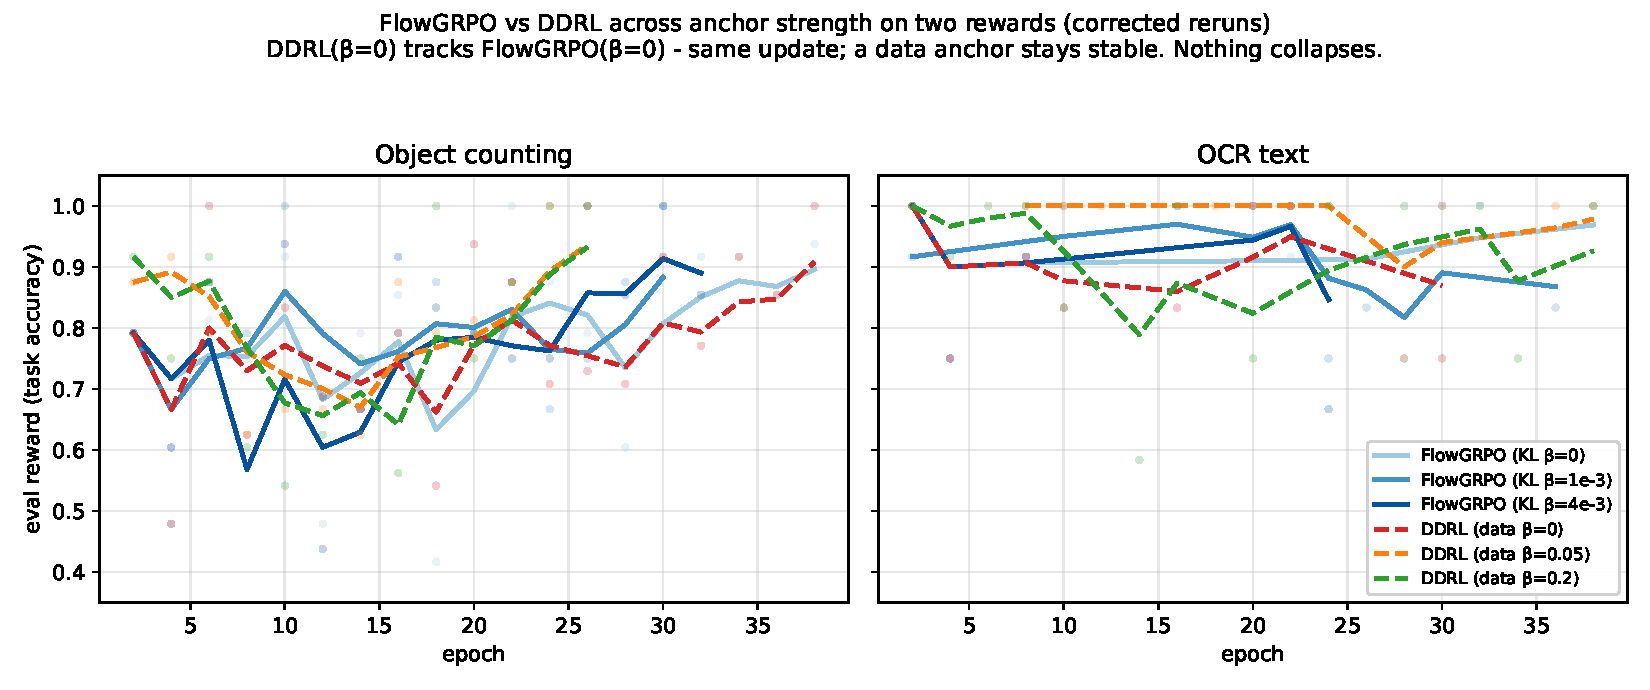
\includegraphics[width=\textwidth]{figures/grid_comparison.pdf}
\caption{Corrected reruns. Faint dots are raw eval points; solid/dashed lines are an
EMA to show the trend. Left (counting) has real headroom: every setting climbs from
$\sim$0.79 toward 1.0, and DDRL(data $\beta{=}0$, red) tracks FlowGRPO(KL $\beta{=}0$,
light blue) - they are the same update. Right (OCR) the base model already scores near
1.0 on these prompts, so there's little room to climb, but nothing collapses at any
anchor strength. This is the exact inverse of my earlier (buggy) grid.}
\label{fig:grid}
\end{figure}

\begin{center}
\small
\begin{tabular}{@{}llccc@{}}
\toprule
\textbf{Reward} & \textbf{Setting} & \textbf{base} & \textbf{peak} & \textbf{final} \\
\midrule
counting & FlowGRPO (KL $\beta{=}0$)     & 0.79 & 1.00 & 0.94 \\
counting & DDRL (data $\beta{=}0$)        & 0.79 & 1.00 & 1.00 \\
counting & DDRL (data $\beta{=}0.05$)     & 0.88 & 1.00 & 1.00 \\
counting & DDRL (data $\beta{=}0.2$)      & 0.92 & 1.00 & 1.00 \\
\midrule
OCR      & FlowGRPO (KL $\beta{=}0$)      & 1.00 & 1.00 & 1.00 \\
OCR      & DDRL (data $\beta{=}0$)        & 1.00 & 1.00 & 0.75$^\dagger$ \\
OCR      & DDRL (data $\beta{=}0.05$)     & 1.00 & 1.00 & 1.00 \\
OCR      & DDRL (data $\beta{=}0.2$)      & 1.00 & 1.00 & 1.00 \\
\bottomrule
\end{tabular}
\end{center}

\noindent Two honest reads. First, the counting row is the clean demonstration: real
headroom, everything climbs, and the $\beta{=}0$ equivalence holds (both start at 0.79
and reach 1.0). Second, OCR is near-saturated at base on these prompts, so the last
values wobble on eval noise ($\dagger$ = a low final on few eval prompts, not a
collapse - the run held $\sim$1.0 throughout). If Haotian wants a \textit{gradual} OCR
climb specifically, we need harder OCR prompts the base model actually fails.

\section{Haotian's critique, and how it resolved}

He raised two points; both were right, and both are now addressed.
\begin{enumerate}
\item \textbf{``FlowGRPO($\beta{=}0$) should perform exactly the same as DDRL($\beta{=}0$),
they're mathematically equivalent - justify the exact same curve.''} Confirmed. My
divergence was the monotonic-transform flag (Sec.~6.3). With it off they run the same
update and track each other (Sec.~9, counting row).
\item \textbf{``With a slightly larger beta, DDRL should show a gradual increase; and
your CFG setting may be inaccurate - try CFG on/off in rollout and training.''} The
gradual, stable climb with the anchor is confirmed on counting. On the ratio issue his
CFG instinct pointed the right direction (the setup \textit{was} invalid) but the
specific cause was the noise level, not CFG (Sec.~5.1): CFG barely moves the ratio
(0.92 on vs 0.94 off), while raising noise 0.1$\to$0.7 takes it to 0.997.
\end{enumerate}

\section{Q\&A drill (say answers out loud)}

\textbf{Q: Why convert the flow ODE to an SDE?} Flow sampling is deterministic - one
prompt, one image, nothing to explore. The SDE injects per-step noise while keeping
the same marginals, turning each step into a Gaussian action with a tractable log-prob.

\textbf{Q: Did the SDE change the model?} No - same distribution over images. Only the
\textit{sampler} became stochastic so RL has something to explore.

\textbf{Q: Why GRPO over PPO?} It drops the critic network. The baseline comes free
from z-scoring a group of samples - roughly half the memory and no critic instability.

\textbf{Q: Why is DDRL($\beta{=}0$) identical to FlowGRPO($\beta{=}0$)?} With both
leashes off, each loss is just the policy-gradient term on the same rollout. Same
computation, so same curve. My earlier divergence was a transform flag that shouldn't
have been on.

\textbf{Q: Why did the monotonic transform collapse it?} $\lambda(A)=-\exp(-A)$ sends
every group-normalized advantage negative, so the PPO update pushes \textit{every}
sampled action's probability down and the policy runs from its own distribution; the
unbounded $\exp$ makes it violent.

\textbf{Q: Your importance ratio was 0.92 - isn't that a bug?} Yes, and I traced it.
Not CFG (0.92 on vs 0.94 off); the cause was low noise (0.1) making the Gaussian
variance tiny, so bf16 rounding between sampling and replay blew up. Noise 0.7 gives
$\rho=0.997$.

\textbf{Q: Why RL over SFT for text rendering?} OCR correctness is sparse, discrete,
non-differentiable, and there's no ideal-image dataset. SFT needs targets and can't
backprop through OCR; RL scores its own samples and reinforces the ones that render
right.

\textbf{Q: Why not DRaFT for OCR?} DRaFT needs a differentiable reward; OCR isn't.

\textbf{Q: How is credit assigned when reward is only at the final image?} Sparse
terminal-reward MDP - the group-normalized final advantage is applied to the log-prob
of every step in the trajectory (a Monte-Carlo return, no discounting since
intermediate rewards are 0).

\textbf{Q: How did you find the bugs?} Gradient-norm assertions and pixel-range checks
on real hardware, not unit tests - e.g. LoRA grad norm was exactly 0 (DRaFT never
trained), decoded images were mostly black (VAE range), and the first-step ratio
$\ne 1.0$ (noise/precision).

\textbf{Q: What would you do differently next?} A held-out eval set (biggest gap),
larger group size, error bars over seeds, and a real OCR benchmark instead of a handful
of prompts.

\section{Formulas to have ready (whiteboard)}

\begin{itemize}
\item \textbf{Flow-matching loss:} $\mathbb E\,\lVert v_\theta(x_t,t)-(x_1-x_0)\rVert^2$,
with $x_1$ = image, $x_0$ = noise, $x_1-x_0$ = target velocity along the straight line.
\item \textbf{GRPO advantage:} $A_i = (r_i - \text{mean})/\text{std}$ within the group.
\item \textbf{PPO clip:} $\min(\rho A,\ \text{clip}(\rho,1{-}\epsilon,1{+}\epsilon)A)$,
$\rho = p_{\text{new}}/p_{\text{old}}$ on the same action.
\item \textbf{KL leash:} $\beta\, D_{\text{KL}}(\pi_\theta \Vert \pi_{\text{ref}})$;
between two Gaussians it scales as $1/\text{noise}^2$.
\item \textbf{DDRL loss:} $\mathcal L_{\text{RL}} + \beta_{\text{data}}\,
\mathcal L_{\text{flow-match(anchor)}}$; at $\beta_{\text{data}}{=}0$ it's just
$\mathcal L_{\text{RL}}$.
\item \textbf{DDRL monotonic transform:} $\lambda(A)=-\exp(-A)$ - only valid with the
anchor on; off by default; leaving it on with $\beta{=}0$ collapses the policy.
\item \textbf{DPO loss:} $-\log\sigma\!\big(\beta[\log\frac{\pi_\theta(w)}{\pi_{\text{ref}}(w)}
- \log\frac{\pi_\theta(l)}{\pi_{\text{ref}}(l)}]\big)$ - push winner up, loser down.
\end{itemize}

\section{Code and architecture - what's in the repo}

Everything lives under \code{src/diffusion\_tinker/}. Names are exact so you can point
at internals in a code review.

\subsection{Package layout}
\code{trainers/} - one \code{*\_trainer.py} + \code{*\_config.py} per method, plus
\code{base\_trainer.py} (abstract base) and \code{base\_config.py}. Six methods:
\code{flowgrpo\_trainer.py}, \code{ddpo\_trainer.py}, \code{ddrl\_trainer.py},
\code{diffusion\_dpo\_trainer.py}, \code{draft\_trainer.py}, \code{sft\_trainer.py}.
\code{core/} - method-agnostic machinery: \code{noise\_strategy.py} (the SDE step +
per-step log-prob, and the flow-matching loss), \code{stat\_tracking.py}
(\code{PerPromptStatTracker}, the group-relative advantage), \code{trajectory.py} (the
rollout container), \code{latent\_utils.py}. \code{models/} - per-architecture
sampling/replay: \code{sd3\_patch.py}, \code{flux\_patch.py}. \code{rewards/} -
\code{base.py} (\code{BaseReward} ABC), \code{resolve.py} (the \code{@register\_reward}
registry), \code{compose.py} (\code{ComposedReward}), and \code{builtin/}
(\code{aesthetic.py}, \code{clip\_score.py}, \code{ocr.py}, \code{count.py},
\code{hps\_v2.py}).

\subsection{The TRL-style API and the abstract base}
\code{BaseDiffusionTrainer} (in \code{trainers/base\_trainer.py}) is an ABC whose
constructor is the public surface and mirrors HuggingFace TRL:
\begin{quote}\code{Trainer(model="stabilityai/...", reward\_funcs="ocr",}\\
\code{~~~~~~~~config=..., train\_prompts=[...]).train()}\end{quote}
The one abstract method a subclass must implement is
\code{\_training\_step(self, trajectory) -> dict}. Everything else - model loading,
rollout, advantages, logging, checkpoint, eval - is inherited. That's the point of the
base class: the online-RL methods differ \textit{only} in \code{\_training\_step}.

\subsection{The shared online-RL update}
FlowGRPO, DDPO, and DDRL share the rollout and the PPO surrogate:
\begin{quote}
\code{ratio = exp(log\_prob\_new - log\_prob\_old)}\\
\code{rl\_loss = mean(max(-adv * ratio,}\\
\code{~~~~~~~~~~~~~~~~-adv * clamp(ratio, 1-clip, 1+clip)))}
\end{quote}
They differ only in (a) the advantage transform in \code{\_compute\_advantages} and
(b) the regularizer added to \code{rl\_loss}. FlowGRPO adds an optional KL to the
LoRA-off reference; DDRL optionally applies the monotonic transform (off by default)
and adds the \code{data\_beta} anchor term; DDPO wraps the surrogate in an outer
PPO-epoch loop. Clean thing to say: same rollout, same PPO surrogate; the method is
the advantage shaping plus the leash.

\subsection{The core SDE machinery}
\code{core/noise\_strategy.py} computes the SDE step-mean and the per-element Gaussian
log-prob of the transition. Sampling stores the transition; replay re-scores that
\textit{same} stored transition through the updated model, so
\code{exp(log\_prob\_new - log\_prob\_old)} is a real importance ratio. One caveat worth
owning: the log-prob is a \textbf{mean over spatial dims, not a sum}, so it's a
numerically-stabilized per-pixel average, not a true trajectory log-density - it behaves
better but isn't the literal probability.

\subsection{The correctness bugs I fixed (point at each in the file)}
This is the differentiating claim - the difference between ``code that runs'' and
``code that trains.'' Each has an exact fix site.
\begin{enumerate}
\item \textbf{DRaFT never trained.} A no-grad warmup cached a detached bf16 copy of the
fp32 LoRA weights, which the grad loop reused, so no gradient reached LoRA (grad norm
exactly 0). Fixed with \code{cache\_enabled=False} in the autocast
(\code{draft\_trainer.py}). Reward then moved 5.9$\to$9.6.
\item \textbf{VAE decode range.} The decoder emits $[-1,1]$; the code clamped to
$[0,1]$ \textit{without} the $/2+0.5$ rescale, so $\sim$55\% of every pixel went black.
This is the bug behind the stale 0.950. (\code{sd3\_patch.py::\_decode\_latents})
\item \textbf{VAE encode range.} $[0,1]$ pixels were fed to an encoder expecting
$[-1,1]$, so SFT/DDRL/DPO trained on mis-scaled latents.
(\code{latent\_utils.py::encode\_to\_latents})
\item \textbf{Biased PPO ratio (precision).} Sampling ran without autocast while replay
ran with it; aligning them (\code{cache\_enabled=False} around the sampling forward)
plus raising the noise level fixed the first-step ratio toward 1.0.
\item \textbf{PEFT API.} The reference-model pass called a wrong-named
\code{disable\_adapter\_layers()} that crashed; fixed to
\code{disable\_adapters()}/\code{enable\_adapters()} in try/finally.
\item \textbf{Monotonic transform on by default in my grid.} $\lambda(A)=-\exp(-A)$ on
group-normalized advantages collapses the policy (Sec.~6.3). Fixed by respecting the
\code{False} default. This is the one that produced my wrong ``DDRL collapses'' result.
\item \textbf{One optimizer step per epoch.} The RL trainers folded a whole batch into
one update, so a long run did only a few dozen steps total. Stepping per mini-batch is
what let the reward actually move.
\item \textbf{Rollout memory.} The previous epoch's trajectory stayed alive into the
next epoch's sampling (2$\times$ peak memory) and the VAE decoded a whole group at once;
freeing per epoch and chunking the decode bounded it.
\end{enumerate}
Common thread for ``how did you find these?'': grad-norm assertions and runtime
pixel-range checks on real GPUs, not unit tests. Several are the same class of failure -
low/mixed-precision handling around the fp32-LoRA / bf16-base split - which is a coherent
story to tell.

\subsection{What you can honestly claim}
Implemented and validated the six trainers (wrote and own each \code{\_training\_step}),
built the SDE log-prob + importance-ratio precision fix (verified by the first-step
ratio $\to 1.0$), the reward system (registry + composition + OCR/counting/aesthetic),
and - the strongest part - found and fixed the correctness bugs that made the difference
between running and training, including catching and correcting my own published DDRL
result. Honest about the scaffold: the SDE math and stat tracker are adapted from
FlowGRPO; it's co-authored with Haotian Ye and Jiaqi Han; no held-out eval, single runs,
single GPU. Say that before anyone asks - it reads as maturity.

\vspace{1em}
\noindent\rule{\linewidth}{0.4pt}\\
\noindent\textit{Code and logs: \url{https://github.com/srijitiyer/diffusion-tinker}}.

\end{document}
